\hypertarget{beschreibung-der-wichtigsten-risiken}{%
\section{Beschreibung der wichtigsten
Risiken}\label{beschreibung-der-wichtigsten-risiken}}

\begin{longtable}[]{@{}llllll@{}}
\toprule
\# & Bezeichnung & Beschreibung des Risikos & P & A & RF\tabularnewline
\midrule
\endhead
1 & Geschäfte & Stellen uns keine Angebote zur Verfügung & 50 & 5 &
250\tabularnewline
2 & Geschäfte2 & Stellen uns keine Angebote zur Verfügung & 50 & 60 &
3000\tabularnewline
\bottomrule
\end{longtable}

\hypertarget{risikoportfolio}{%
\section{Risikoportfolio}\label{risikoportfolio}}

\begin{figure}
\centering
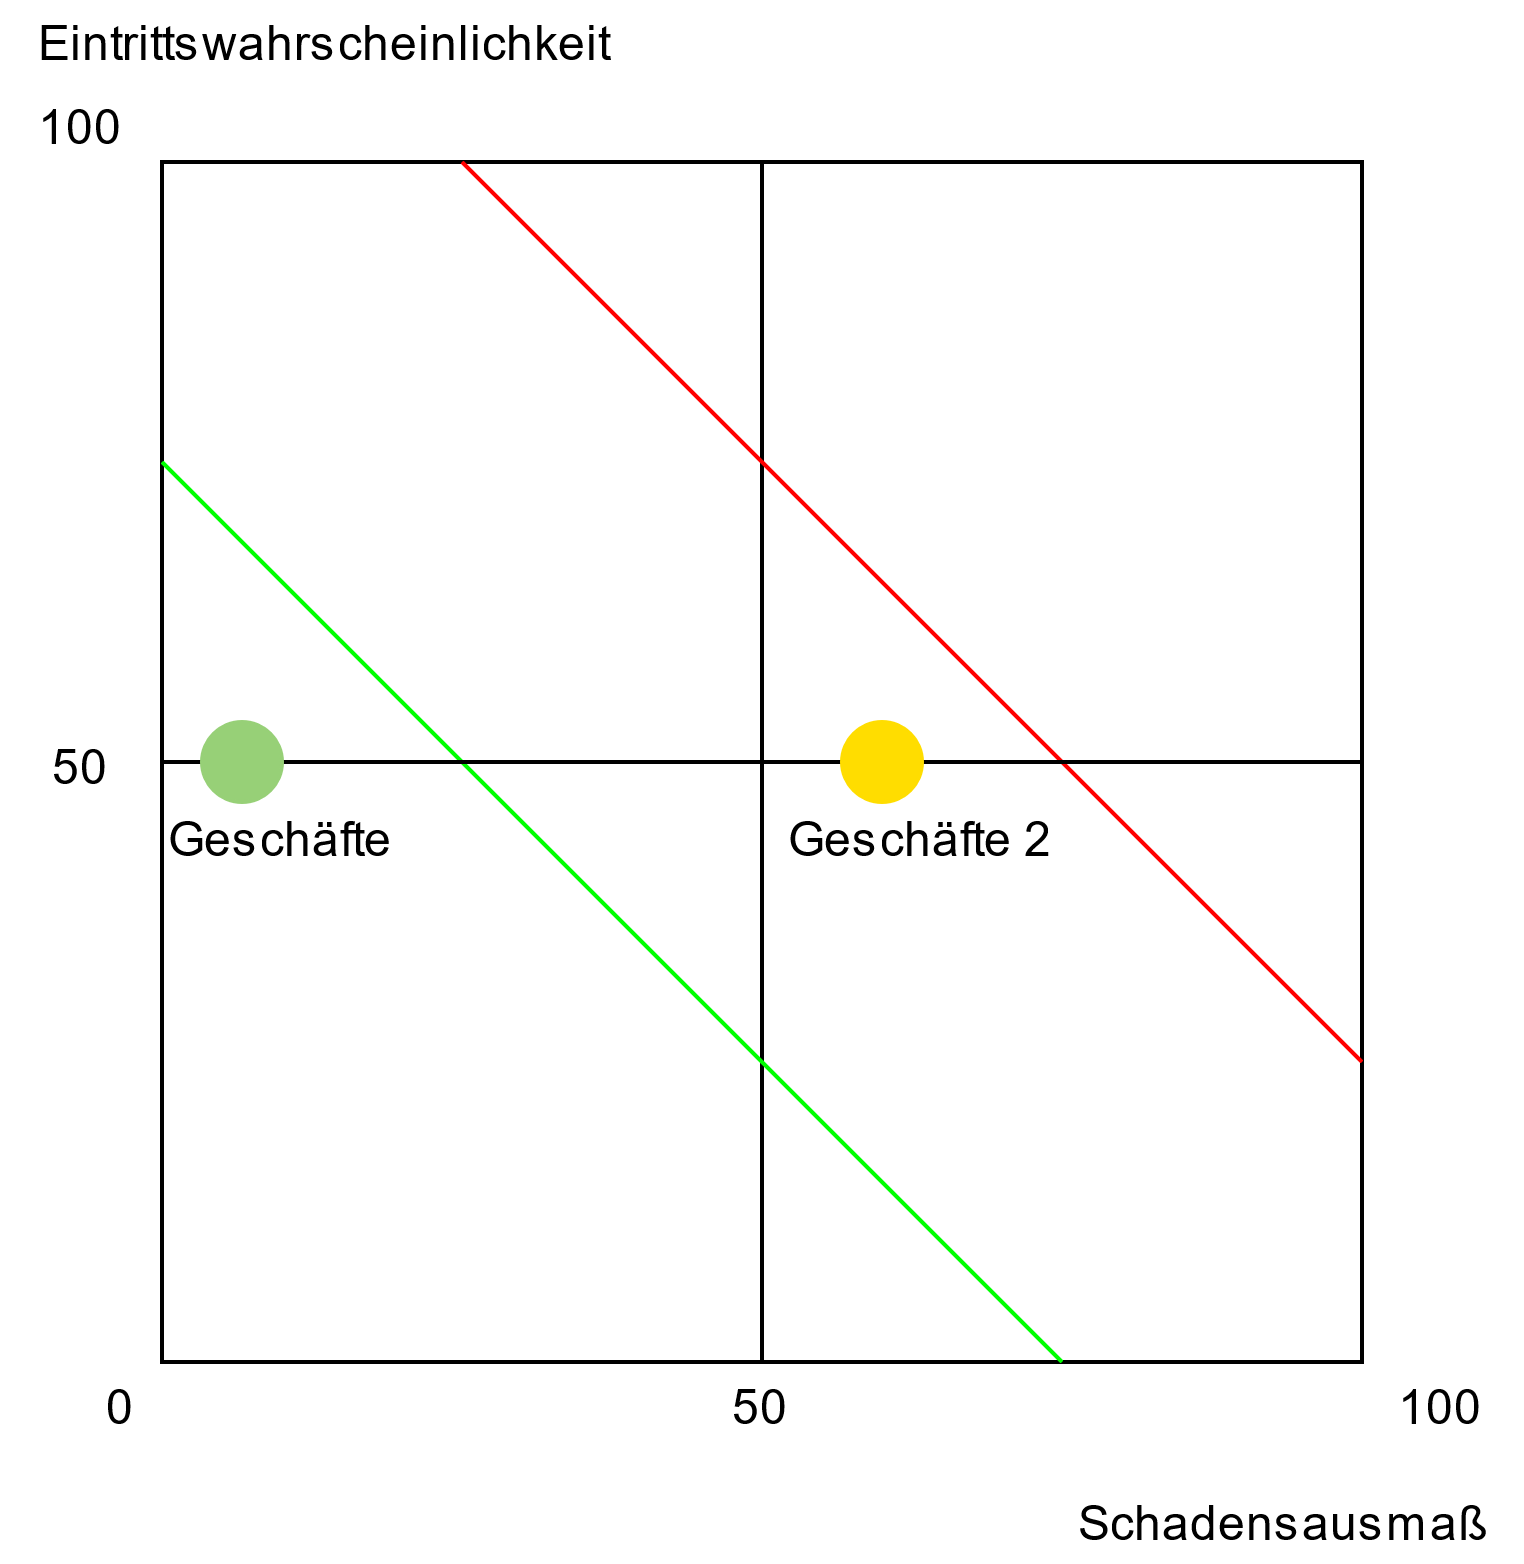
\includegraphics[width=2cm,height=\textheight]{images/doja/risikoanalyse.png}
\caption{Bild des Risikoportfolios\label{King Bild}}
\end{figure}

\hypertarget{risiko-gegenmauxdfnahmen}{%
\section{Risiko Gegenmaßnahmen}\label{risiko-gegenmauxdfnahmen}}

\begin{longtable}[]{@{}lll@{}}
\toprule
\# & Bezeichnung & Gegenmaßnahme\tabularnewline
\midrule
\endhead
1 & Geschäfte & Angebote werden selbst eingetragen\tabularnewline
2 & Geschäfte2 & Wir müssen die User-Daten selbst organisieren und
einteilen\tabularnewline
\bottomrule
\end{longtable}
